\documentclass[1p]{elsarticle_modified}
%\bibliographystyle{elsarticle-num}

%\usepackage[colorlinks]{hyperref}
%\usepackage{abbrmath_seonhwa} %\Abb, \Ascr, \Acal ,\Abf, \Afrak
\usepackage{amsfonts}
\usepackage{amssymb}
\usepackage{amsmath}
\usepackage{amsthm}
\usepackage{scalefnt}
\usepackage{amsbsy}
\usepackage{kotex}
\usepackage{caption}
\usepackage{subfig}
\usepackage{color}
\usepackage{graphicx}
\usepackage{xcolor} %% white, black, red, green, blue, cyan, magenta, yellow
\usepackage{float}
\usepackage{setspace}
\usepackage{hyperref}

\usepackage{tikz}
\usetikzlibrary{arrows}

\usepackage{multirow}
\usepackage{array} % fixed length table
\usepackage{hhline}

%%%%%%%%%%%%%%%%%%%%%
\makeatletter
\renewcommand*\env@matrix[1][\arraystretch]{%
	\edef\arraystretch{#1}%
	\hskip -\arraycolsep
	\let\@ifnextchar\new@ifnextchar
	\array{*\c@MaxMatrixCols c}}
\makeatother %https://tex.stackexchange.com/questions/14071/how-can-i-increase-the-line-spacing-in-a-matrix
%%%%%%%%%%%%%%%

\usepackage[normalem]{ulem}

\newcommand{\msout}[1]{\ifmmode\text{\sout{\ensuremath{#1}}}\else\sout{#1}\fi}
%SOURCE: \msout is \stkout macro in https://tex.stackexchange.com/questions/20609/strikeout-in-math-mode

\newcommand{\cancel}[1]{
	\ifmmode
	{\color{red}\msout{#1}}
	\else
	{\color{red}\sout{#1}}
	\fi
}

\newcommand{\add}[1]{
	{\color{blue}\uwave{#1}}
}

\newcommand{\replace}[2]{
	\ifmmode
	{\color{red}\msout{#1}}{\color{blue}\uwave{#2}}
	\else
	{\color{red}\sout{#1}}{\color{blue}\uwave{#2}}
	\fi
}

\newcommand{\Sol}{\mathcal{S}} %segment
\newcommand{\D}{D} %diagram
\newcommand{\A}{\mathcal{A}} %arc


%%%%%%%%%%%%%%%%%%%%%%%%%%%%%5 test

\def\sl{\operatorname{\textup{SL}}(2,\Cbb)}
\def\psl{\operatorname{\textup{PSL}}(2,\Cbb)}
\def\quan{\mkern 1mu \triangleright \mkern 1mu}

\theoremstyle{definition}
\newtheorem{thm}{Theorem}[section]
\newtheorem{prop}[thm]{Proposition}
\newtheorem{lem}[thm]{Lemma}
\newtheorem{ques}[thm]{Question}
\newtheorem{cor}[thm]{Corollary}
\newtheorem{defn}[thm]{Definition}
\newtheorem{exam}[thm]{Example}
\newtheorem{rmk}[thm]{Remark}
\newtheorem{alg}[thm]{Algorithm}

\newcommand{\I}{\sqrt{-1}}
\begin{document}

%\begin{frontmatter}
%
%\title{Boundary parabolic representations of knots up to 8 crossings}
%
%%% Group authors per affiliation:
%\author{Yunhi Cho} 
%\address{Department of Mathematics, University of Seoul, Seoul, Korea}
%\ead{yhcho@uos.ac.kr}
%
%
%\author{Seonhwa Kim} %\fnref{s_kim}}
%\address{Center for Geometry and Physics, Institute for Basic Science, Pohang, 37673, Korea}
%\ead{ryeona17@ibs.re.kr}
%
%\author{Hyuk Kim}
%\address{Department of Mathematical Sciences, Seoul National University, Seoul 08826, Korea}
%\ead{hyukkim@snu.ac.kr}
%
%\author{Seokbeom Yoon}
%\address{Department of Mathematical Sciences, Seoul National University, Seoul, 08826,  Korea}
%\ead{sbyoon15@snu.ac.kr}
%
%\begin{abstract}
%We find all boundary parabolic representation of knots up to 8 crossings.
%
%\end{abstract}
%\begin{keyword}
%    \MSC[2010] 57M25 
%\end{keyword}
%
%\end{frontmatter}

%\linenumbers
%\tableofcontents
%
\newcommand\colored[1]{\textcolor{white}{\rule[-0.35ex]{0.8em}{1.4ex}}\kern-0.8em\color{red} #1}%
%\newcommand\colored[1]{\textcolor{white}{ #1}\kern-2.17ex	\textcolor{white}{ #1}\kern-1.81ex	\textcolor{white}{ #1}\kern-2.15ex\color{red}#1	}

{\Large $\underline{12a_{0746}~(K12a_{0746})}$}

\setlength{\tabcolsep}{10pt}
\renewcommand{\arraystretch}{1.6}
\vspace{1cm}\begin{tabular}{m{100pt}>{\centering\arraybackslash}m{274pt}}
\multirow{5}{120pt}{
	\centering
	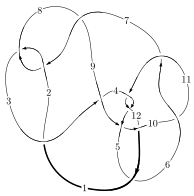
\includegraphics[width=112pt]{../../../GIT/diagram.site/Diagrams/png/1547_12a_0746.png}\\
\ \ \ A knot diagram\footnotemark}&
\allowdisplaybreaks
\textbf{Linearized knot diagam} \\
\cline{2-2}
 &
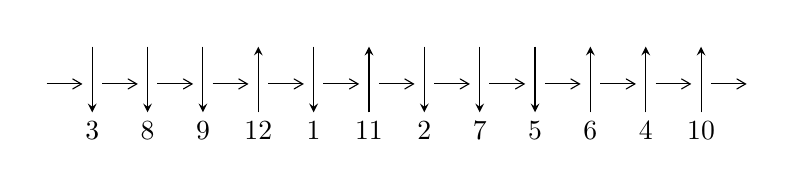
\begin{tikzpicture}[x=20pt, y=17pt]
	% nodes
	\node (C0) at (0, 0) {};
	\node (C1) at (1, 0) {};
	\node (C1U) at (1, +1) {};
	\node (C1D) at (1, -1) {3};

	\node (C2) at (2, 0) {};
	\node (C2U) at (2, +1) {};
	\node (C2D) at (2, -1) {8};

	\node (C3) at (3, 0) {};
	\node (C3U) at (3, +1) {};
	\node (C3D) at (3, -1) {9};

	\node (C4) at (4, 0) {};
	\node (C4U) at (4, +1) {};
	\node (C4D) at (4, -1) {12};

	\node (C5) at (5, 0) {};
	\node (C5U) at (5, +1) {};
	\node (C5D) at (5, -1) {1};

	\node (C6) at (6, 0) {};
	\node (C6U) at (6, +1) {};
	\node (C6D) at (6, -1) {11};

	\node (C7) at (7, 0) {};
	\node (C7U) at (7, +1) {};
	\node (C7D) at (7, -1) {2};

	\node (C8) at (8, 0) {};
	\node (C8U) at (8, +1) {};
	\node (C8D) at (8, -1) {7};

	\node (C9) at (9, 0) {};
	\node (C9U) at (9, +1) {};
	\node (C9D) at (9, -1) {5};

	\node (C10) at (10, 0) {};
	\node (C10U) at (10, +1) {};
	\node (C10D) at (10, -1) {6};

	\node (C11) at (11, 0) {};
	\node (C11U) at (11, +1) {};
	\node (C11D) at (11, -1) {4};

	\node (C12) at (12, 0) {};
	\node (C12U) at (12, +1) {};
	\node (C12D) at (12, -1) {10};
	\node (C13) at (13, 0) {};

	% arrows
	\draw[->,>={angle 60}]
	(C0) edge (C1) (C1) edge (C2) (C2) edge (C3) (C3) edge (C4) (C4) edge (C5) (C5) edge (C6) (C6) edge (C7) (C7) edge (C8) (C8) edge (C9) (C9) edge (C10) (C10) edge (C11) (C11) edge (C12) (C12) edge (C13) ;	\draw[->,>=stealth]
	(C1U) edge (C1D) (C2U) edge (C2D) (C3U) edge (C3D) (C4D) edge (C4U) (C5U) edge (C5D) (C6D) edge (C6U) (C7U) edge (C7D) (C8U) edge (C8D) (C9U) edge (C9D) (C10D) edge (C10U) (C11D) edge (C11U) (C12D) edge (C12U) ;
	\end{tikzpicture} \\
\hhline{~~} \\& 
\textbf{Solving Sequence} \\ \cline{2-2} 
 &
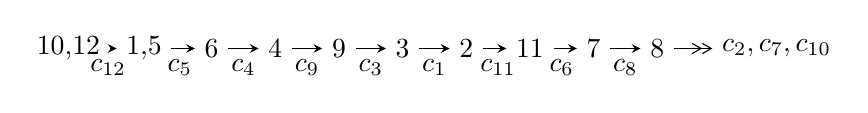
\begin{tikzpicture}[x=23pt, y=7pt]
	% node
	\node (A0) at (-1/8, 0) {10,12};
	\node (A1) at (17/16, 0) {1,5};
	\node (A2) at (17/8, 0) {6};
	\node (A3) at (25/8, 0) {4};
	\node (A4) at (33/8, 0) {9};
	\node (A5) at (41/8, 0) {3};
	\node (A6) at (49/8, 0) {2};
	\node (A7) at (57/8, 0) {11};
	\node (A8) at (65/8, 0) {7};
	\node (A9) at (73/8, 0) {8};
	\node (C1) at (1/2, -1) {$c_{12}$};
	\node (C2) at (13/8, -1) {$c_{5}$};
	\node (C3) at (21/8, -1) {$c_{4}$};
	\node (C4) at (29/8, -1) {$c_{9}$};
	\node (C5) at (37/8, -1) {$c_{3}$};
	\node (C6) at (45/8, -1) {$c_{1}$};
	\node (C7) at (53/8, -1) {$c_{11}$};
	\node (C8) at (61/8, -1) {$c_{6}$};
	\node (C9) at (69/8, -1) {$c_{8}$};
	\node (A10) at (11, 0) {$c_{2},c_{7},c_{10}$};

	% edge
	\draw[->,>=stealth]	
	(A0) edge (A1) (A1) edge (A2) (A2) edge (A3) (A3) edge (A4) (A4) edge (A5) (A5) edge (A6) (A6) edge (A7) (A7) edge (A8) (A8) edge (A9) ;
	\draw[->>,>={angle 60}]	
	(A9) edge (A10);
\end{tikzpicture} \\ 

\end{tabular} \\

\footnotetext{
The image of knot diagram is generated by the software ``\textbf{Draw programme}" developed by Andrew Bartholomew(\url{http://www.layer8.co.uk/maths/draw/index.htm\#Running-draw}), where we modified some parts for our purpose(\url{https://github.com/CATsTAILs/LinksPainter}).
}\phantom \\ \newline 
\centering \textbf{Ideals for irreducible components\footnotemark of $X_{\text{par}}$} 
 
\begin{align*}
I^u_{1}&=\langle 
1872295 u^{40}+66648388 u^{39}+\cdots+16384 b+56849186816,\\
\phantom{I^u_{1}}&\phantom{= \langle  }-1204339 u^{40}-38682066 u^{39}+\cdots+32768 a+33461256192,\\
\phantom{I^u_{1}}&\phantom{= \langle  }u^{41}+36 u^{40}+\cdots+753664 u+32768\rangle \\
I^u_{2}&=\langle 
-1.34031\times10^{114} a^{29} u^{2}+8.19598\times10^{113} a^{28} u^{2}+\cdots-1.54708\times10^{113} a+1.81464\times10^{113},\\
\phantom{I^u_{2}}&\phantom{= \langle  }a^{29} u^2-3 a^{28} u^2+\cdots+376065 a-197787,\;u^3- u^2+1\rangle \\
I^u_{3}&=\langle 
3 u^{22}-27 u^{21}+\cdots+b+8,\;10 u^{22}-108 u^{21}+\cdots+a+11,\;u^{23}-11 u^{22}+\cdots+6 u^2-1\rangle \\
\\
\end{align*}
\raggedright * 3 irreducible components of $\dim_{\mathbb{C}}=0$, with total 154 representations.\\
\footnotetext{All coefficients of polynomials are rational numbers. But the coefficients are sometimes approximated in decimal forms when there is not enough margin.}
\newpage
\renewcommand{\arraystretch}{1}
\centering \section*{I. $I^u_{1}= \langle 1.87\times10^{6} u^{40}+6.66\times10^{7} u^{39}+\cdots+1.64\times10^{4} b+5.68\times10^{10},\;-1.20\times10^{6} u^{40}-3.87\times10^{7} u^{39}+\cdots+3.28\times10^{4} a+3.35\times10^{10},\;u^{41}+36 u^{40}+\cdots+753664 u+32768 \rangle$}
\flushleft \textbf{(i) Arc colorings}\\
\begin{tabular}{m{7pt} m{180pt} m{7pt} m{180pt} }
\flushright $a_{10}=$&$\begin{pmatrix}0\\u\end{pmatrix}$ \\
\flushright $a_{12}=$&$\begin{pmatrix}1\\0\end{pmatrix}$ \\
\flushright $a_{1}=$&$\begin{pmatrix}1\\- u^2\end{pmatrix}$ \\
\flushright $a_{5}=$&$\begin{pmatrix}36.7535 u^{40}+1180.48 u^{39}+\cdots-2.15671\times10^{7} u-1.02116\times10^{6}\\-114.276 u^{40}-4067.89 u^{39}+\cdots-7.75799\times10^{7} u-3469799\end{pmatrix}$ \\
\flushright $a_{6}=$&$\begin{pmatrix}-105.890 u^{40}-3697.76 u^{39}+\cdots-5.02880\times10^{7} u-2.22550\times10^{6}\\188.678 u^{40}+6690.58 u^{39}+\cdots+1.11377\times10^{8} u+4948929\end{pmatrix}$ \\
\flushright $a_{4}=$&$\begin{pmatrix}151.029 u^{40}+5248.38 u^{39}+\cdots+5.60128\times10^{7} u+2.44864\times10^{6}\\-114.276 u^{40}-4067.89 u^{39}+\cdots-7.75799\times10^{7} u-3469799\end{pmatrix}$ \\
\flushright $a_{9}=$&$\begin{pmatrix}-0.996094 u^{40}-34.8672 u^{39}+\cdots-720833 u-32767.5\\-\frac{1}{128} u^{39}-\frac{17}{64} u^{38}+\cdots-\frac{5631}{2} u-128\end{pmatrix}$ \\
\flushright $a_{3}=$&$\begin{pmatrix}-70.0146 u^{40}-2541.25 u^{39}+\cdots-6.41108\times10^{7} u-2.91215\times10^{6}\\-162.712 u^{40}-5404.01 u^{39}+\cdots+4.14685\times10^{6} u+284302\end{pmatrix}$ \\
\flushright $a_{2}=$&$\begin{pmatrix}-3.80273 u^{40}-133.703 u^{39}+\cdots+1.67651\times10^{6} u+92160.5\\-7.14063 u^{40}-242.551 u^{39}+\cdots-524672. u-18112\end{pmatrix}$ \\
\flushright $a_{11}=$&$\begin{pmatrix}-\frac{1}{256} u^{40}-\frac{17}{128} u^{39}+\cdots-64 u+\frac{1}{2}\\\frac{1}{128} u^{40}+\frac{35}{128} u^{39}+\cdots+\frac{5889}{2} u+128\end{pmatrix}$ \\
\flushright $a_{7}=$&$\begin{pmatrix}15.9481 u^{40}+686.796 u^{39}+\cdots+4.13601\times10^{7} u+1877871\\187.066 u^{40}+6323.84 u^{39}+\cdots+2.36552\times10^{7} u+956542\end{pmatrix}$ \\
\flushright $a_{8}=$&$\begin{pmatrix}-4.98438 u^{40}-175.410 u^{39}+\cdots-3.13728\times10^{6} u-140671\\-0.902344 u^{40}-29.0820 u^{39}+\cdots-594048 u-29568\end{pmatrix}$\\&\end{tabular}
\flushleft \textbf{(ii) Obstruction class $= -1$}\\~\\
\flushleft \textbf{(iii) Cusp Shapes $= \frac{338489}{4096} u^{40}+\frac{6389611}{2048} u^{39}+\cdots+101047790 u+4578666$}\\~\\
\newpage\renewcommand{\arraystretch}{1}
\flushleft \textbf{(iv) u-Polynomials at the component}\newline \\
\begin{tabular}{m{50pt}|m{274pt}}
Crossings & \hspace{64pt}u-Polynomials at each crossing \\
\hline $$\begin{aligned}c_{1},c_{8}\end{aligned}$$&$\begin{aligned}
&u^{41}+13 u^{40}+\cdots+160 u+64
\end{aligned}$\\
\hline $$\begin{aligned}c_{2},c_{7}\end{aligned}$$&$\begin{aligned}
&u^{41}+7 u^{40}+\cdots-56 u-8
\end{aligned}$\\
\hline $$\begin{aligned}c_{3}\end{aligned}$$&$\begin{aligned}
&u^{41}-7 u^{40}+\cdots-90808 u-82952
\end{aligned}$\\
\hline $$\begin{aligned}c_{4},c_{6},c_{10}\\c_{11}\end{aligned}$$&$\begin{aligned}
&u^{41}- u^{40}+\cdots+u+1
\end{aligned}$\\
\hline $$\begin{aligned}c_{5},c_{9}\end{aligned}$$&$\begin{aligned}
&u^{41}-3 u^{39}+\cdots+11 u^2-1
\end{aligned}$\\
\hline $$\begin{aligned}c_{12}\end{aligned}$$&$\begin{aligned}
&u^{41}+36 u^{40}+\cdots+753664 u+32768
\end{aligned}$\\
\hline
\end{tabular}\\~\\
\newpage\renewcommand{\arraystretch}{1}
\flushleft \textbf{(v) Riley Polynomials at the component}\newline \\
\begin{tabular}{m{50pt}|m{274pt}}
Crossings & \hspace{64pt}Riley Polynomials at each crossing \\
\hline $$\begin{aligned}c_{1},c_{8}\end{aligned}$$&$\begin{aligned}
&y^{41}+27 y^{40}+\cdots-34304 y-4096
\end{aligned}$\\
\hline $$\begin{aligned}c_{2},c_{7}\end{aligned}$$&$\begin{aligned}
&y^{41}-13 y^{40}+\cdots+160 y-64
\end{aligned}$\\
\hline $$\begin{aligned}c_{3}\end{aligned}$$&$\begin{aligned}
&y^{41}-9 y^{40}+\cdots+128877877536 y-6881034304
\end{aligned}$\\
\hline $$\begin{aligned}c_{4},c_{6},c_{10}\\c_{11}\end{aligned}$$&$\begin{aligned}
&y^{41}-29 y^{40}+\cdots-11 y-1
\end{aligned}$\\
\hline $$\begin{aligned}c_{5},c_{9}\end{aligned}$$&$\begin{aligned}
&y^{41}-6 y^{40}+\cdots+22 y-1
\end{aligned}$\\
\hline $$\begin{aligned}c_{12}\end{aligned}$$&$\begin{aligned}
&y^{41}-12 y^{40}+\cdots+4294967296 y-1073741824
\end{aligned}$\\
\hline
\end{tabular}\\~\\
\newpage\flushleft \textbf{(vi) Complex Volumes and Cusp Shapes}
$$\begin{array}{c|c|c}  
\text{Solutions to }I^u_{1}& \I (\text{vol} + \sqrt{-1}CS) & \text{Cusp shape}\\
 \hline 
\begin{aligned}
u &= -0.494014 + 0.701063 I \\
a &= \phantom{-}0.409463 + 1.060830 I \\
b &= \phantom{-}0.312502 + 0.783120 I\end{aligned}
 & -2.26568 + 4.00425 I & \phantom{-0.000000 } 0 \\ \hline\begin{aligned}
u &= -0.494014 - 0.701063 I \\
a &= \phantom{-}0.409463 - 1.060830 I \\
b &= \phantom{-}0.312502 - 0.783120 I\end{aligned}
 & -2.26568 - 4.00425 I & \phantom{-0.000000 } 0 \\ \hline\begin{aligned}
u &= -0.679352 + 0.497133 I \\
a &= \phantom{-}0.52438 + 1.38712 I \\
b &= -0.003532 + 0.738483 I\end{aligned}
 & -1.28548 - 7.83101 I & \phantom{-0.000000 } 0 \\ \hline\begin{aligned}
u &= -0.679352 - 0.497133 I \\
a &= \phantom{-}0.52438 - 1.38712 I \\
b &= -0.003532 - 0.738483 I\end{aligned}
 & -1.28548 + 7.83101 I & \phantom{-0.000000 } 0 \\ \hline\begin{aligned}
u &= -0.595725 + 0.586119 I \\
a &= \phantom{-}0.465409 + 1.248190 I \\
b &= \phantom{-}0.131910 + 0.781629 I\end{aligned}
 & -5.73006 - 1.89264 I & \phantom{-0.000000 } 0 \\ \hline\begin{aligned}
u &= -0.595725 - 0.586119 I \\
a &= \phantom{-}0.465409 - 1.248190 I \\
b &= \phantom{-}0.131910 - 0.781629 I\end{aligned}
 & -5.73006 + 1.89264 I & \phantom{-0.000000 } 0 \\ \hline\begin{aligned}
u &= -0.638217 + 0.462865 I \\
a &= -0.46096 - 1.41417 I \\
b &= -0.024247 - 0.688483 I\end{aligned}
 & -0.16397 - 2.42178 I & \phantom{-0.000000 } 0 \\ \hline\begin{aligned}
u &= -0.638217 - 0.462865 I \\
a &= -0.46096 + 1.41417 I \\
b &= -0.024247 + 0.688483 I\end{aligned}
 & -0.16397 + 2.42178 I & \phantom{-0.000000 } 0 \\ \hline\begin{aligned}
u &= -0.381047 + 0.557336 I \\
a &= -0.196071 - 1.164500 I \\
b &= -0.261553 - 0.610371 I\end{aligned}
 & -1.177580 - 0.730802 I & \phantom{-0.000000 } 0 \\ \hline\begin{aligned}
u &= -0.381047 - 0.557336 I \\
a &= -0.196071 + 1.164500 I \\
b &= -0.261553 + 0.610371 I\end{aligned}
 & -1.177580 + 0.730802 I & \phantom{-0.000000 } 0\\
 \hline 
 \end{array}$$\newpage$$\begin{array}{c|c|c}  
\text{Solutions to }I^u_{1}& \I (\text{vol} + \sqrt{-1}CS) & \text{Cusp shape}\\
 \hline 
\begin{aligned}
u &= -0.220982 + 0.635974 I \\
a &= -0.066893 - 0.971313 I \\
b &= -0.383287 - 0.536330 I\end{aligned}
 & -1.196420 - 0.686597 I & \phantom{-0.000000 } 0 \\ \hline\begin{aligned}
u &= -0.220982 - 0.635974 I \\
a &= -0.066893 + 0.971313 I \\
b &= -0.383287 + 0.536330 I\end{aligned}
 & -1.196420 + 0.686597 I & \phantom{-0.000000 } 0 \\ \hline\begin{aligned}
u &= -0.535272 + 0.041843 I \\
a &= -0.03970 - 1.81222 I \\
b &= -0.004595 - 0.454090 I\end{aligned}
 & \phantom{-}2.83170 - 2.66585 I & \phantom{-0.000000 } 0 \\ \hline\begin{aligned}
u &= -0.535272 - 0.041843 I \\
a &= -0.03970 + 1.81222 I \\
b &= -0.004595 + 0.454090 I\end{aligned}
 & \phantom{-}2.83170 + 2.66585 I & \phantom{-0.000000 } 0 \\ \hline\begin{aligned}
u &= -0.03812 + 1.48635 I \\
a &= -0.193307 - 0.307958 I \\
b &= -0.856986 - 0.426230 I\end{aligned}
 & -1.58172 + 4.75393 I & \phantom{-0.000000 } 0 \\ \hline\begin{aligned}
u &= -0.03812 - 1.48635 I \\
a &= -0.193307 + 0.307958 I \\
b &= -0.856986 + 0.426230 I\end{aligned}
 & -1.58172 - 4.75393 I & \phantom{-0.000000 } 0 \\ \hline\begin{aligned}
u &= -1.29282 + 0.89016 I \\
a &= -0.120939 - 1.059210 I \\
b &= \phantom{-}1.44499 - 0.60902 I\end{aligned}
 & \phantom{-}7.5896 - 18.8889 I & \phantom{-0.000000 } 0 \\ \hline\begin{aligned}
u &= -1.29282 - 0.89016 I \\
a &= -0.120939 + 1.059210 I \\
b &= \phantom{-}1.44499 + 0.60902 I\end{aligned}
 & \phantom{-}7.5896 + 18.8889 I & \phantom{-0.000000 } 0 \\ \hline\begin{aligned}
u &= -1.31919 + 0.85653 I \\
a &= -0.190725 - 1.009320 I \\
b &= \phantom{-}1.35678 - 0.58313 I\end{aligned}
 & \phantom{-}1.73884 - 12.70420 I & \phantom{-0.000000 } 0 \\ \hline\begin{aligned}
u &= -1.31919 - 0.85653 I \\
a &= -0.190725 + 1.009320 I \\
b &= \phantom{-}1.35678 + 0.58313 I\end{aligned}
 & \phantom{-}1.73884 + 12.70420 I & \phantom{-0.000000 } 0\\
 \hline 
 \end{array}$$\newpage$$\begin{array}{c|c|c}  
\text{Solutions to }I^u_{1}& \I (\text{vol} + \sqrt{-1}CS) & \text{Cusp shape}\\
 \hline 
\begin{aligned}
u &= -1.30409 + 0.89542 I \\
a &= \phantom{-}0.112178 + 1.034570 I \\
b &= -1.44431 + 0.58076 I\end{aligned}
 & \phantom{-}8.6919 - 12.9687 I & \phantom{-0.000000 } 0 \\ \hline\begin{aligned}
u &= -1.30409 - 0.89542 I \\
a &= \phantom{-}0.112178 - 1.034570 I \\
b &= -1.44431 - 0.58076 I\end{aligned}
 & \phantom{-}8.6919 + 12.9687 I & \phantom{-0.000000 } 0 \\ \hline\begin{aligned}
u &= -1.39385 + 0.82232 I \\
a &= -0.249205 - 0.882711 I \\
b &= \phantom{-}1.265940 - 0.478660 I\end{aligned}
 & \phantom{-}3.40814 - 5.76593 I & \phantom{-0.000000 } 0 \\ \hline\begin{aligned}
u &= -1.39385 - 0.82232 I \\
a &= -0.249205 + 0.882711 I \\
b &= \phantom{-}1.265940 + 0.478660 I\end{aligned}
 & \phantom{-}3.40814 + 5.76593 I & \phantom{-0.000000 } 0 \\ \hline\begin{aligned}
u &= -1.36265 + 0.87524 I \\
a &= \phantom{-}0.161547 + 0.929339 I \\
b &= -1.35943 + 0.49662 I\end{aligned}
 & \phantom{-}6.04010 - 9.92499 I & \phantom{-0.000000 } 0 \\ \hline\begin{aligned}
u &= -1.36265 - 0.87524 I \\
a &= \phantom{-}0.161547 - 0.929339 I \\
b &= -1.35943 - 0.49662 I\end{aligned}
 & \phantom{-}6.04010 + 9.92499 I & \phantom{-0.000000 } 0 \\ \hline\begin{aligned}
u &= \phantom{-}0.91303 + 1.42279 I \\
a &= -0.038442 + 0.198861 I \\
b &= \phantom{-}0.788921 + 0.209788 I\end{aligned}
 & \phantom{-}1.61353 + 1.37467 I & \phantom{-0.000000 } 0 \\ \hline\begin{aligned}
u &= \phantom{-}0.91303 - 1.42279 I \\
a &= -0.038442 - 0.198861 I \\
b &= \phantom{-}0.788921 - 0.209788 I\end{aligned}
 & \phantom{-}1.61353 - 1.37467 I & \phantom{-0.000000 } 0 \\ \hline\begin{aligned}
u &= -1.46025 + 0.98895 I \\
a &= \phantom{-}0.034082 + 0.742902 I \\
b &= -1.40055 + 0.29202 I\end{aligned}
 & \phantom{-}11.9449 - 8.5283 I & \phantom{-0.000000 } 0 \\ \hline\begin{aligned}
u &= -1.46025 - 0.98895 I \\
a &= \phantom{-}0.034082 - 0.742902 I \\
b &= -1.40055 - 0.29202 I\end{aligned}
 & \phantom{-}11.9449 + 8.5283 I & \phantom{-0.000000 } 0\\
 \hline 
 \end{array}$$\newpage$$\begin{array}{c|c|c}  
\text{Solutions to }I^u_{1}& \I (\text{vol} + \sqrt{-1}CS) & \text{Cusp shape}\\
 \hline 
\begin{aligned}
u &= -1.74926 + 0.43149 I \\
a &= \phantom{-}0.535712 + 0.368017 I \\
b &= -0.999153 + 0.163720 I\end{aligned}
 & \phantom{-}1.06152 - 7.56290 I & \phantom{-0.000000 } 0 \\ \hline\begin{aligned}
u &= -1.74926 - 0.43149 I \\
a &= \phantom{-}0.535712 - 0.368017 I \\
b &= -0.999153 - 0.163720 I\end{aligned}
 & \phantom{-}1.06152 + 7.56290 I & \phantom{-0.000000 } 0 \\ \hline\begin{aligned}
u &= -1.50520 + 1.01021 I \\
a &= -0.033661 - 0.682040 I \\
b &= \phantom{-}1.376430 - 0.245763 I\end{aligned}
 & \phantom{-}11.74060 - 2.35789 I & \phantom{-0.000000 } 0 \\ \hline\begin{aligned}
u &= -1.50520 - 1.01021 I \\
a &= -0.033661 + 0.682040 I \\
b &= \phantom{-}1.376430 + 0.245763 I\end{aligned}
 & \phantom{-}11.74060 + 2.35789 I & \phantom{-0.000000 } 0 \\ \hline\begin{aligned}
u &= -1.85197\phantom{ +0.000000I} \\
a &= \phantom{-}0.605999\phantom{ +0.000000I} \\
b &= -0.956151\phantom{ +0.000000I}\end{aligned}
 & -2.89727\phantom{ +0.000000I} & \phantom{-0.000000 } 0 \\ \hline\begin{aligned}
u &= -0.51953 + 1.79430 I \\
a &= -0.311173 - 0.112547 I \\
b &= -1.071610 - 0.412248 I\end{aligned}
 & \phantom{-}5.01069 + 10.47520 I & \phantom{-0.000000 } 0 \\ \hline\begin{aligned}
u &= -0.51953 - 1.79430 I \\
a &= -0.311173 + 0.112547 I \\
b &= -1.071610 + 0.412248 I\end{aligned}
 & \phantom{-}5.01069 - 10.47520 I & \phantom{-0.000000 } 0 \\ \hline\begin{aligned}
u &= -0.48632 + 1.95335 I \\
a &= \phantom{-}0.259519 + 0.091738 I \\
b &= \phantom{-}1.059950 + 0.359083 I\end{aligned}
 & \phantom{-}5.99467 + 4.35481 I & \phantom{-0.000000 } 0 \\ \hline\begin{aligned}
u &= -0.48632 - 1.95335 I \\
a &= \phantom{-}0.259519 - 0.091738 I \\
b &= \phantom{-}1.059950 - 0.359083 I\end{aligned}
 & \phantom{-}5.99467 - 4.35481 I & \phantom{-0.000000 } 0 \\ \hline\begin{aligned}
u &= -2.01115 + 0.42725 I \\
a &= -0.404223 - 0.233635 I \\
b &= \phantom{-}1.049910 - 0.089496 I\end{aligned}
 & \phantom{-}3.11118 - 2.16671 I & \phantom{-0.000000 } 0\\
 \hline 
 \end{array}$$\newpage$$\begin{array}{c|c|c}  
\text{Solutions to }I^u_{1}& \I (\text{vol} + \sqrt{-1}CS) & \text{Cusp shape}\\
 \hline 
\begin{aligned}
u &= -2.01115 - 0.42725 I \\
a &= -0.404223 + 0.233635 I \\
b &= \phantom{-}1.049910 + 0.089496 I\end{aligned}
 & \phantom{-}3.11118 + 2.16671 I & \phantom{-0.000000 } 0\\
 \hline 
 \end{array}$$\newpage\newpage\renewcommand{\arraystretch}{1}
\centering \section*{II. $I^u_{2}= \langle -1.34\times10^{114} a^{29} u^{2}+8.20\times10^{113} a^{28} u^{2}+\cdots-1.55\times10^{113} a+1.81\times10^{113},\;a^{29} u^2-3 a^{28} u^2+\cdots+376065 a-197787,\;u^3- u^2+1 \rangle$}
\flushleft \textbf{(i) Arc colorings}\\
\begin{tabular}{m{7pt} m{180pt} m{7pt} m{180pt} }
\flushright $a_{10}=$&$\begin{pmatrix}0\\u\end{pmatrix}$ \\
\flushright $a_{12}=$&$\begin{pmatrix}1\\0\end{pmatrix}$ \\
\flushright $a_{1}=$&$\begin{pmatrix}1\\- u^2\end{pmatrix}$ \\
\flushright $a_{5}=$&$\begin{pmatrix}a\\23.4794 a^{29} u^{2}-14.3576 a^{28} u^{2}+\cdots+2.71016 a-3.17887\end{pmatrix}$ \\
\flushright $a_{6}=$&$\begin{pmatrix}-23.4794 a^{29} u^{2}+14.3576 a^{28} u^{2}+\cdots-1.71016 a+3.17887\\-27.3348 a^{29} u^{2}+27.3560 a^{28} u^{2}+\cdots+3.17365 a-5.12591\end{pmatrix}$ \\
\flushright $a_{4}=$&$\begin{pmatrix}-23.4794 a^{29} u^{2}+14.3576 a^{28} u^{2}+\cdots-1.71016 a+3.17887\\23.4794 a^{29} u^{2}-14.3576 a^{28} u^{2}+\cdots+2.71016 a-3.17887\end{pmatrix}$ \\
\flushright $a_{9}=$&$\begin{pmatrix}a^2 u\\-3.17106 a^{29} u^{2}-0.698057 a^{28} u^{2}+\cdots+1.92192 a+1.25518\end{pmatrix}$ \\
\flushright $a_{3}=$&$\begin{pmatrix}-31.9841 a^{29} u^{2}+23.7739 a^{28} u^{2}+\cdots-2.37529 a+3.16621\\-36.2658 a^{29} u^{2}+53.0390 a^{28} u^{2}+\cdots-1.06179 a-3.97206\end{pmatrix}$ \\
\flushright $a_{2}=$&$\begin{pmatrix}6.78809 a^{29} u^{2}+9.35682 a^{28} u^{2}+\cdots+1.47987 a+0.523084\\94.6666 a^{29} u^{2}-99.3068 a^{28} u^{2}+\cdots+1.75209 a+1.13744\end{pmatrix}$ \\
\flushright $a_{11}=$&$\begin{pmatrix}16.4889 a^{29} u^{2}-11.1613 a^{28} u^{2}+\cdots+0.398085 a-0.546245\\-25.9756 a^{29} u^{2}+15.4354 a^{28} u^{2}+\cdots+0.595930 a+0.830310\end{pmatrix}$ \\
\flushright $a_{7}=$&$\begin{pmatrix}-39.5709 a^{29} u^{2}+24.8065 a^{28} u^{2}+\cdots+7.53533 a-1.91582\\-22.4865 a^{29} u^{2}+33.8142 a^{28} u^{2}+\cdots-14.1437 a-0.0624415\end{pmatrix}$ \\
\flushright $a_{8}=$&$\begin{pmatrix}10.3333 a^{29} u^{2}-21.1205 a^{28} u^{2}+\cdots+6.37351 a+1.67760\\-75.5055 a^{29} u^{2}+80.2424 a^{28} u^{2}+\cdots-6.87074 a-2.17822\end{pmatrix}$\\&\end{tabular}
\flushleft \textbf{(ii) Obstruction class $= -1$}\\~\\
\flushleft \textbf{(iii) Cusp Shapes $= 52.9371 a^{29} u^{2}-16.2200 a^{28} u^{2}+\cdots-9.05243 a+0.463477$}\\~\\
\newpage\renewcommand{\arraystretch}{1}
\flushleft \textbf{(iv) u-Polynomials at the component}\newline \\
\begin{tabular}{m{50pt}|m{274pt}}
Crossings & \hspace{64pt}u-Polynomials at each crossing \\
\hline $$\begin{aligned}c_{1},c_{8}\end{aligned}$$&$\begin{aligned}
&(u^{15}+5 u^{14}+\cdots+12 u^3+1)^{6}
\end{aligned}$\\
\hline $$\begin{aligned}c_{2},c_{7}\end{aligned}$$&$\begin{aligned}
&(u^{15}- u^{14}+\cdots+2 u-1)^{6}
\end{aligned}$\\
\hline $$\begin{aligned}c_{3}\end{aligned}$$&$\begin{aligned}
&(u^{15}+u^{14}+\cdots-4 u-1)^{6}
\end{aligned}$\\
\hline $$\begin{aligned}c_{4},c_{6},c_{10}\\c_{11}\end{aligned}$$&$\begin{aligned}
&u^{90}+u^{89}+\cdots+119082 u-20779
\end{aligned}$\\
\hline $$\begin{aligned}c_{5},c_{9}\end{aligned}$$&$\begin{aligned}
&u^{90}+3 u^{89}+\cdots+464 u-43
\end{aligned}$\\
\hline $$\begin{aligned}c_{12}\end{aligned}$$&$\begin{aligned}
&(u^3- u^2+1)^{30}
\end{aligned}$\\
\hline
\end{tabular}\\~\\
\newpage\renewcommand{\arraystretch}{1}
\flushleft \textbf{(v) Riley Polynomials at the component}\newline \\
\begin{tabular}{m{50pt}|m{274pt}}
Crossings & \hspace{64pt}Riley Polynomials at each crossing \\
\hline $$\begin{aligned}c_{1},c_{8}\end{aligned}$$&$\begin{aligned}
&(y^{15}+11 y^{14}+\cdots-84 y^2-1)^{6}
\end{aligned}$\\
\hline $$\begin{aligned}c_{2},c_{7}\end{aligned}$$&$\begin{aligned}
&(y^{15}-5 y^{14}+\cdots+12 y^3-1)^{6}
\end{aligned}$\\
\hline $$\begin{aligned}c_{3}\end{aligned}$$&$\begin{aligned}
&(y^{15}- y^{14}+\cdots+16 y-1)^{6}
\end{aligned}$\\
\hline $$\begin{aligned}c_{4},c_{6},c_{10}\\c_{11}\end{aligned}$$&$\begin{aligned}
&y^{90}-69 y^{89}+\cdots-21058454840 y+431766841
\end{aligned}$\\
\hline $$\begin{aligned}c_{5},c_{9}\end{aligned}$$&$\begin{aligned}
&y^{90}+23 y^{89}+\cdots+88800 y+1849
\end{aligned}$\\
\hline $$\begin{aligned}c_{12}\end{aligned}$$&$\begin{aligned}
&(y^3- y^2+2 y-1)^{30}
\end{aligned}$\\
\hline
\end{tabular}\\~\\
\newpage\flushleft \textbf{(vi) Complex Volumes and Cusp Shapes}
$$\begin{array}{c|c|c}  
\text{Solutions to }I^u_{2}& \I (\text{vol} + \sqrt{-1}CS) & \text{Cusp shape}\\
 \hline 
\begin{aligned}
u &= \phantom{-}0.877439 + 0.744862 I \\
a &= -0.198485 - 0.968997 I \\
b &= -0.694930 - 1.099660 I\end{aligned}
 & \phantom{-}4.92757 - 1.26387 I & \phantom{-}3.53451 + 0.17150 I \\ \hline\begin{aligned}
u &= \phantom{-}0.877439 + 0.744862 I \\
a &= \phantom{-}0.371784 - 0.910068 I \\
b &= -0.912624 - 0.535628 I\end{aligned}
 & \phantom{-}0.08992 + 4.90214 I & -3.33798 - 5.65067 I \\ \hline\begin{aligned}
u &= \phantom{-}0.877439 + 0.744862 I \\
a &= \phantom{-}0.159762 + 0.960463 I \\
b &= \phantom{-}0.595959 + 1.123610 I\end{aligned}
 & \phantom{-}5.44406 + 4.33335 I & \phantom{-}4.64158 - 5.71992 I \\ \hline\begin{aligned}
u &= \phantom{-}0.877439 + 0.744862 I \\
a &= -0.838607 - 0.592740 I \\
b &= -0.355737 + 0.306163 I\end{aligned}
 & \phantom{-}5.44406 + 1.32289 I & \phantom{-}4.64158 - 0.23897 I \\ \hline\begin{aligned}
u &= \phantom{-}0.877439 + 0.744862 I \\
a &= \phantom{-}0.909407 - 0.268588 I \\
b &= -0.365280 - 0.653329 I\end{aligned}
 & \phantom{-}2.93698 - 6.38968 I & \phantom{-}0.34485 + 4.41190 I \\ \hline\begin{aligned}
u &= \phantom{-}0.877439 + 0.744862 I \\
a &= \phantom{-}0.132786 - 0.935412 I \\
b &= -0.022537 - 1.398180 I\end{aligned}
 & \phantom{-}2.93698 + 12.04590 I & \phantom{-}0.34485 - 10.37079 I \\ \hline\begin{aligned}
u &= \phantom{-}0.877439 + 0.744862 I \\
a &= -0.100613 + 0.931593 I \\
b &= \phantom{-}0.072834 + 1.359600 I\end{aligned}
 & \phantom{-}3.89372 + 6.34664 I & \phantom{-}2.20327 - 5.56972 I \\ \hline\begin{aligned}
u &= \phantom{-}0.877439 + 0.744862 I \\
a &= -0.281606 - 0.878991 I \\
b &= -0.862552 - 0.726604 I\end{aligned}
 & \phantom{-}0.48639 + 2.82812 I & -2.07315 - 2.97945 I \\ \hline\begin{aligned}
u &= \phantom{-}0.877439 + 0.744862 I \\
a &= \phantom{-}0.858189 + 0.699478 I \\
b &= \phantom{-}0.467845 - 0.303279 I\end{aligned}
 & \phantom{-}4.92757 + 6.92011 I & \phantom{-}3.53451 - 6.13039 I \\ \hline\begin{aligned}
u &= \phantom{-}0.877439 + 0.744862 I \\
a &= -0.860296 + 0.181110 I \\
b &= \phantom{-}0.318140 + 0.586816 I\end{aligned}
 & \phantom{-}3.89372 - 0.69040 I & \phantom{-}2.20327 - 0.38918 I\\
 \hline 
 \end{array}$$\newpage$$\begin{array}{c|c|c}  
\text{Solutions to }I^u_{2}& \I (\text{vol} + \sqrt{-1}CS) & \text{Cusp shape}\\
 \hline 
\begin{aligned}
u &= \phantom{-}0.877439 + 0.744862 I \\
a &= -0.371348 - 0.789042 I \\
b &= -1.183520 - 0.597870 I\end{aligned}
 & \phantom{-}4.92757 + 6.92011 I & \phantom{-}3.53451 - 6.13039 I \\ \hline\begin{aligned}
u &= \phantom{-}0.877439 + 0.744862 I \\
a &= \phantom{-}0.572239 + 0.977295 I \\
b &= \phantom{-}0.746751 + 0.022825 I\end{aligned}
 & \phantom{-}0.48639 + 2.82812 I & -2.00000 - 2.97945 I \\ \hline\begin{aligned}
u &= \phantom{-}0.877439 + 0.744862 I \\
a &= \phantom{-}0.137577 - 0.832217 I \\
b &= \phantom{-}0.089498 - 1.235180 I\end{aligned}
 & -2.29749 + 6.43153 I & -5.67348 - 7.45617 I \\ \hline\begin{aligned}
u &= \phantom{-}0.877439 + 0.744862 I \\
a &= \phantom{-}0.357793 + 0.741926 I \\
b &= \phantom{-}1.187160 + 0.517480 I\end{aligned}
 & \phantom{-}5.44406 + 1.32289 I & \phantom{-}4.64158 - 0.23897 I \\ \hline\begin{aligned}
u &= \phantom{-}0.877439 + 0.744862 I \\
a &= -0.004665 + 0.807225 I \\
b &= \phantom{-}0.093049 + 1.047120 I\end{aligned}
 & \phantom{-}1.55950 + 4.48897 I & \phantom{-}2.00066 - 6.94350 I \\ \hline\begin{aligned}
u &= \phantom{-}0.877439 + 0.744862 I \\
a &= \phantom{-}0.633092 - 0.463259 I \\
b &= -0.595731 - 0.536286 I\end{aligned}
 & -2.29749 - 0.77528 I & -5.67348 + 1.49727 I \\ \hline\begin{aligned}
u &= \phantom{-}0.877439 + 0.744862 I \\
a &= -0.236441 + 1.237330 I \\
b &= \phantom{-}1.087060 + 0.511062 I\end{aligned}
 & \phantom{-}0.089924 + 0.754105 I & -3.33798 + 0. I\phantom{ +0.000000I} \\ \hline\begin{aligned}
u &= \phantom{-}0.877439 + 0.744862 I \\
a &= -0.045040 - 1.346060 I \\
b &= -1.144440 - 0.356431 I\end{aligned}
 & \phantom{-}1.55950 + 4.48897 I & \phantom{-0.000000 } 0. - 6.94350 I \\ \hline\begin{aligned}
u &= \phantom{-}0.877439 + 0.744862 I \\
a &= \phantom{-}0.121715 - 0.636837 I \\
b &= \phantom{-}0.270487 - 0.931692 I\end{aligned}
 & \phantom{-}0.089924 + 0.754105 I & -3.33798 - 0.30823 I \\ \hline\begin{aligned}
u &= \phantom{-}0.877439 + 0.744862 I \\
a &= \phantom{-}0.53100 + 1.33570 I \\
b &= \phantom{-}1.084130 + 0.016709 I\end{aligned}
 & \phantom{-}4.92757 - 1.26387 I & \phantom{-0.000000 } 0\\
 \hline 
 \end{array}$$\newpage$$\begin{array}{c|c|c}  
\text{Solutions to }I^u_{2}& \I (\text{vol} + \sqrt{-1}CS) & \text{Cusp shape}\\
 \hline 
\begin{aligned}
u &= \phantom{-}0.877439 + 0.744862 I \\
a &= -0.45129 - 1.37089 I \\
b &= -1.119650 - 0.076995 I\end{aligned}
 & \phantom{-}5.44406 + 4.33335 I & \phantom{-0.000000 } 0 \\ \hline\begin{aligned}
u &= \phantom{-}0.877439 + 0.744862 I \\
a &= -0.012024 + 0.552750 I \\
b &= \phantom{-}0.920975 + 0.296695 I\end{aligned}
 & \phantom{-}1.55950 + 1.16728 I & \phantom{-}2.00066 + 0.98460 I \\ \hline\begin{aligned}
u &= \phantom{-}0.877439 + 0.744862 I \\
a &= -0.10536 + 1.49620 I \\
b &= \phantom{-}1.237800 + 0.443667 I\end{aligned}
 & -2.29749 + 6.43153 I & \phantom{-0.000000 } 0 \\ \hline\begin{aligned}
u &= \phantom{-}0.877439 + 0.744862 I \\
a &= -0.388709 - 0.214363 I \\
b &= -1.194610 + 0.112491 I\end{aligned}
 & \phantom{-}2.93698 - 6.38968 I & \phantom{-}0.34485 + 4.41190 I \\ \hline\begin{aligned}
u &= \phantom{-}0.877439 + 0.744862 I \\
a &= \phantom{-}0.349082 + 0.272090 I \\
b &= \phantom{-}1.170340 - 0.032932 I\end{aligned}
 & \phantom{-}3.89372 - 0.69040 I & \phantom{-}2.20327 - 0.38918 I \\ \hline\begin{aligned}
u &= \phantom{-}0.877439 + 0.744862 I \\
a &= -0.03053 - 1.60206 I \\
b &= -1.305370 - 0.357996 I\end{aligned}
 & \phantom{-}3.89372 + 6.34664 I & \phantom{-0.000000 } 0 \\ \hline\begin{aligned}
u &= \phantom{-}0.877439 + 0.744862 I \\
a &= -0.354568 - 0.154720 I \\
b &= \phantom{-}0.296292 + 0.020701 I\end{aligned}
 & \phantom{-}1.55950 + 1.16728 I & \phantom{-}2.00066 + 0.98460 I \\ \hline\begin{aligned}
u &= \phantom{-}0.877439 + 0.744862 I \\
a &= -0.098435 + 0.363229 I \\
b &= -0.508129 + 0.572146 I\end{aligned}
 & \phantom{-}0.08992 + 4.90214 I & -3.33798 - 5.65067 I \\ \hline\begin{aligned}
u &= \phantom{-}0.877439 + 0.744862 I \\
a &= -0.01217 + 1.63528 I \\
b &= \phantom{-}1.326900 + 0.386050 I\end{aligned}
 & \phantom{-}2.93698 + 12.04590 I & \phantom{-0.000000 } 0 \\ \hline\begin{aligned}
u &= \phantom{-}0.877439 + 0.744862 I \\
a &= -0.204433 - 0.044838 I \\
b &= -0.915203 + 0.211781 I\end{aligned}
 & -2.29749 - 0.77528 I & -5.67348 + 1.49727 I\\
 \hline 
 \end{array}$$\newpage$$\begin{array}{c|c|c}  
\text{Solutions to }I^u_{2}& \I (\text{vol} + \sqrt{-1}CS) & \text{Cusp shape}\\
 \hline 
\begin{aligned}
u &= \phantom{-}0.877439 - 0.744862 I \\
a &= -0.198485 + 0.968997 I \\
b &= -0.694930 + 1.099660 I\end{aligned}
 & \phantom{-}4.92757 + 1.26387 I & \phantom{-}3.53451 - 0.17150 I \\ \hline\begin{aligned}
u &= \phantom{-}0.877439 - 0.744862 I \\
a &= \phantom{-}0.371784 + 0.910068 I \\
b &= -0.912624 + 0.535628 I\end{aligned}
 & \phantom{-}0.08992 - 4.90214 I & -3.33798 + 5.65067 I \\ \hline\begin{aligned}
u &= \phantom{-}0.877439 - 0.744862 I \\
a &= \phantom{-}0.159762 - 0.960463 I \\
b &= \phantom{-}0.595959 - 1.123610 I\end{aligned}
 & \phantom{-}5.44406 - 4.33335 I & \phantom{-}4.64158 + 5.71992 I \\ \hline\begin{aligned}
u &= \phantom{-}0.877439 - 0.744862 I \\
a &= -0.838607 + 0.592740 I \\
b &= -0.355737 - 0.306163 I\end{aligned}
 & \phantom{-}5.44406 - 1.32289 I & \phantom{-}4.64158 + 0.23897 I \\ \hline\begin{aligned}
u &= \phantom{-}0.877439 - 0.744862 I \\
a &= \phantom{-}0.909407 + 0.268588 I \\
b &= -0.365280 + 0.653329 I\end{aligned}
 & \phantom{-}2.93698 + 6.38968 I & \phantom{-}0.34485 - 4.41190 I \\ \hline\begin{aligned}
u &= \phantom{-}0.877439 - 0.744862 I \\
a &= \phantom{-}0.132786 + 0.935412 I \\
b &= -0.022537 + 1.398180 I\end{aligned}
 & \phantom{-}2.93698 - 12.04590 I & \phantom{-}0.34485 + 10.37079 I \\ \hline\begin{aligned}
u &= \phantom{-}0.877439 - 0.744862 I \\
a &= -0.100613 - 0.931593 I \\
b &= \phantom{-}0.072834 - 1.359600 I\end{aligned}
 & \phantom{-}3.89372 - 6.34664 I & \phantom{-}2.20327 + 5.56972 I \\ \hline\begin{aligned}
u &= \phantom{-}0.877439 - 0.744862 I \\
a &= -0.281606 + 0.878991 I \\
b &= -0.862552 + 0.726604 I\end{aligned}
 & \phantom{-}0.48639 - 2.82812 I & -2.07315 + 2.97945 I \\ \hline\begin{aligned}
u &= \phantom{-}0.877439 - 0.744862 I \\
a &= \phantom{-}0.858189 - 0.699478 I \\
b &= \phantom{-}0.467845 + 0.303279 I\end{aligned}
 & \phantom{-}4.92757 - 6.92011 I & \phantom{-}3.53451 + 6.13039 I \\ \hline\begin{aligned}
u &= \phantom{-}0.877439 - 0.744862 I \\
a &= -0.860296 - 0.181110 I \\
b &= \phantom{-}0.318140 - 0.586816 I\end{aligned}
 & \phantom{-}3.89372 + 0.69040 I & \phantom{-}2.20327 + 0.38918 I\\
 \hline 
 \end{array}$$\newpage$$\begin{array}{c|c|c}  
\text{Solutions to }I^u_{2}& \I (\text{vol} + \sqrt{-1}CS) & \text{Cusp shape}\\
 \hline 
\begin{aligned}
u &= \phantom{-}0.877439 - 0.744862 I \\
a &= -0.371348 + 0.789042 I \\
b &= -1.183520 + 0.597870 I\end{aligned}
 & \phantom{-}4.92757 - 6.92011 I & \phantom{-}3.53451 + 6.13039 I \\ \hline\begin{aligned}
u &= \phantom{-}0.877439 - 0.744862 I \\
a &= \phantom{-}0.572239 - 0.977295 I \\
b &= \phantom{-}0.746751 - 0.022825 I\end{aligned}
 & \phantom{-}0.48639 - 2.82812 I & -2.00000 + 2.97945 I \\ \hline\begin{aligned}
u &= \phantom{-}0.877439 - 0.744862 I \\
a &= \phantom{-}0.137577 + 0.832217 I \\
b &= \phantom{-}0.089498 + 1.235180 I\end{aligned}
 & -2.29749 - 6.43153 I & -5.67348 + 7.45617 I \\ \hline\begin{aligned}
u &= \phantom{-}0.877439 - 0.744862 I \\
a &= \phantom{-}0.357793 - 0.741926 I \\
b &= \phantom{-}1.187160 - 0.517480 I\end{aligned}
 & \phantom{-}5.44406 - 1.32289 I & \phantom{-}4.64158 + 0.23897 I \\ \hline\begin{aligned}
u &= \phantom{-}0.877439 - 0.744862 I \\
a &= -0.004665 - 0.807225 I \\
b &= \phantom{-}0.093049 - 1.047120 I\end{aligned}
 & \phantom{-}1.55950 - 4.48897 I & \phantom{-}2.00066 + 6.94350 I \\ \hline\begin{aligned}
u &= \phantom{-}0.877439 - 0.744862 I \\
a &= \phantom{-}0.633092 + 0.463259 I \\
b &= -0.595731 + 0.536286 I\end{aligned}
 & -2.29749 + 0.77528 I & -5.67348 - 1.49727 I \\ \hline\begin{aligned}
u &= \phantom{-}0.877439 - 0.744862 I \\
a &= -0.236441 - 1.237330 I \\
b &= \phantom{-}1.087060 - 0.511062 I\end{aligned}
 & \phantom{-}0.089924 - 0.754105 I & -3.33798 + 0. I\phantom{ +0.000000I} \\ \hline\begin{aligned}
u &= \phantom{-}0.877439 - 0.744862 I \\
a &= -0.045040 + 1.346060 I \\
b &= -1.144440 + 0.356431 I\end{aligned}
 & \phantom{-}1.55950 - 4.48897 I & \phantom{-0.000000 -}0. + 6.94350 I \\ \hline\begin{aligned}
u &= \phantom{-}0.877439 - 0.744862 I \\
a &= \phantom{-}0.121715 + 0.636837 I \\
b &= \phantom{-}0.270487 + 0.931692 I\end{aligned}
 & \phantom{-}0.089924 - 0.754105 I & -3.33798 + 0.30823 I \\ \hline\begin{aligned}
u &= \phantom{-}0.877439 - 0.744862 I \\
a &= \phantom{-}0.53100 - 1.33570 I \\
b &= \phantom{-}1.084130 - 0.016709 I\end{aligned}
 & \phantom{-}4.92757 + 1.26387 I & \phantom{-0.000000 } 0\\
 \hline 
 \end{array}$$\newpage$$\begin{array}{c|c|c}  
\text{Solutions to }I^u_{2}& \I (\text{vol} + \sqrt{-1}CS) & \text{Cusp shape}\\
 \hline 
\begin{aligned}
u &= \phantom{-}0.877439 - 0.744862 I \\
a &= -0.45129 + 1.37089 I \\
b &= -1.119650 + 0.076995 I\end{aligned}
 & \phantom{-}5.44406 - 4.33335 I & \phantom{-0.000000 } 0 \\ \hline\begin{aligned}
u &= \phantom{-}0.877439 - 0.744862 I \\
a &= -0.012024 - 0.552750 I \\
b &= \phantom{-}0.920975 - 0.296695 I\end{aligned}
 & \phantom{-}1.55950 - 1.16728 I & \phantom{-}2.00066 - 0.98460 I \\ \hline\begin{aligned}
u &= \phantom{-}0.877439 - 0.744862 I \\
a &= -0.10536 - 1.49620 I \\
b &= \phantom{-}1.237800 - 0.443667 I\end{aligned}
 & -2.29749 - 6.43153 I & \phantom{-0.000000 } 0 \\ \hline\begin{aligned}
u &= \phantom{-}0.877439 - 0.744862 I \\
a &= -0.388709 + 0.214363 I \\
b &= -1.194610 - 0.112491 I\end{aligned}
 & \phantom{-}2.93698 + 6.38968 I & \phantom{-}0.34485 - 4.41190 I \\ \hline\begin{aligned}
u &= \phantom{-}0.877439 - 0.744862 I \\
a &= \phantom{-}0.349082 - 0.272090 I \\
b &= \phantom{-}1.170340 + 0.032932 I\end{aligned}
 & \phantom{-}3.89372 + 0.69040 I & \phantom{-}2.20327 + 0.38918 I \\ \hline\begin{aligned}
u &= \phantom{-}0.877439 - 0.744862 I \\
a &= -0.03053 + 1.60206 I \\
b &= -1.305370 + 0.357996 I\end{aligned}
 & \phantom{-}3.89372 - 6.34664 I & \phantom{-0.000000 } 0 \\ \hline\begin{aligned}
u &= \phantom{-}0.877439 - 0.744862 I \\
a &= -0.354568 + 0.154720 I \\
b &= \phantom{-}0.296292 - 0.020701 I\end{aligned}
 & \phantom{-}1.55950 - 1.16728 I & \phantom{-}2.00066 - 0.98460 I \\ \hline\begin{aligned}
u &= \phantom{-}0.877439 - 0.744862 I \\
a &= -0.098435 - 0.363229 I \\
b &= -0.508129 - 0.572146 I\end{aligned}
 & \phantom{-}0.08992 - 4.90214 I & -3.33798 + 5.65067 I \\ \hline\begin{aligned}
u &= \phantom{-}0.877439 - 0.744862 I \\
a &= -0.01217 - 1.63528 I \\
b &= \phantom{-}1.326900 - 0.386050 I\end{aligned}
 & \phantom{-}2.93698 - 12.04590 I & \phantom{-0.000000 } 0 \\ \hline\begin{aligned}
u &= \phantom{-}0.877439 - 0.744862 I \\
a &= -0.204433 + 0.044838 I \\
b &= -0.915203 - 0.211781 I\end{aligned}
 & -2.29749 + 0.77528 I & -5.67348 - 1.49727 I\\
 \hline 
 \end{array}$$\newpage$$\begin{array}{c|c|c}  
\text{Solutions to }I^u_{2}& \I (\text{vol} + \sqrt{-1}CS) & \text{Cusp shape}\\
 \hline 
\begin{aligned}
u &= -0.754878\phantom{ +0.000000I} \\
a &= -0.403780 + 1.129560 I \\
b &= \phantom{-}1.43132 + 0.52104 I\end{aligned}
 & \phantom{-}5.69708 + 1.66084 I & \phantom{-}8.52993 - 3.96405 I \\ \hline\begin{aligned}
u &= -0.754878\phantom{ +0.000000I} \\
a &= -0.403780 - 1.129560 I \\
b &= \phantom{-}1.43132 - 0.52104 I\end{aligned}
 & \phantom{-}5.69708 - 1.66084 I & \phantom{-}8.52993 + 3.96405 I \\ \hline\begin{aligned}
u &= -0.754878\phantom{ +0.000000I} \\
a &= -0.092959 + 1.224570 I \\
b &= \phantom{-}1.50634 + 0.79741 I\end{aligned}
 & \phantom{-}8.03130 + 3.51852 I & \phantom{-}8.73253 - 2.59027 I \\ \hline\begin{aligned}
u &= -0.754878\phantom{ +0.000000I} \\
a &= -0.092959 - 1.224570 I \\
b &= \phantom{-}1.50634 - 0.79741 I\end{aligned}
 & \phantom{-}8.03130 - 3.51852 I & \phantom{-}8.73253 + 2.59027 I \\ \hline\begin{aligned}
u &= -0.754878\phantom{ +0.000000I} \\
a &= \phantom{-}0.069471 + 1.279600 I \\
b &= -1.47299 + 0.85189 I\end{aligned}
 & \phantom{-}7.07456 - 9.21780 I & \phantom{-}6.87411 + 7.39135 I \\ \hline\begin{aligned}
u &= -0.754878\phantom{ +0.000000I} \\
a &= \phantom{-}0.069471 - 1.279600 I \\
b &= -1.47299 - 0.85189 I\end{aligned}
 & \phantom{-}7.07456 + 9.21780 I & \phantom{-}6.87411 - 7.39135 I \\ \hline\begin{aligned}
u &= -0.754878\phantom{ +0.000000I} \\
a &= -0.126876 + 0.612176 I \\
b &= \phantom{-}1.83118 + 0.39406 I\end{aligned}
 & \phantom{-}9.58164 + 1.50523 I & \phantom{-}11.17084 - 2.74048 I \\ \hline\begin{aligned}
u &= -0.754878\phantom{ +0.000000I} \\
a &= -0.126876 - 0.612176 I \\
b &= \phantom{-}1.83118 - 0.39406 I\end{aligned}
 & \phantom{-}9.58164 - 1.50523 I & \phantom{-}11.17084 + 2.74048 I \\ \hline\begin{aligned}
u &= -0.754878\phantom{ +0.000000I} \\
a &= \phantom{-}0.243400 + 1.354700 I \\
b &= -1.31484 + 0.72928 I\end{aligned}
 & \phantom{-}1.84009 - 3.60340 I & \phantom{-0.000000 -}0. + 4.47672 I \\ \hline\begin{aligned}
u &= -0.754878\phantom{ +0.000000I} \\
a &= \phantom{-}0.243400 - 1.354700 I \\
b &= -1.31484 - 0.72928 I\end{aligned}
 & \phantom{-}1.84009 + 3.60340 I & \phantom{-0.000000 } 0. - 4.47672 I\\
 \hline 
 \end{array}$$\newpage$$\begin{array}{c|c|c}  
\text{Solutions to }I^u_{2}& \I (\text{vol} + \sqrt{-1}CS) & \text{Cusp shape}\\
 \hline 
\begin{aligned}
u &= -0.754878\phantom{ +0.000000I} \\
a &= \phantom{-}0.093933 + 0.494243 I \\
b &= -1.88877 + 0.32776 I\end{aligned}
 & \phantom{-}9.06515 + 4.09199 I & \phantom{-}10.06378 - 3.15094 I \\ \hline\begin{aligned}
u &= -0.754878\phantom{ +0.000000I} \\
a &= \phantom{-}0.093933 - 0.494243 I \\
b &= -1.88877 - 0.32776 I\end{aligned}
 & \phantom{-}9.06515 - 4.09199 I & \phantom{-}10.06378 + 3.15094 I \\ \hline\begin{aligned}
u &= -0.754878\phantom{ +0.000000I} \\
a &= \phantom{-}0.397055\phantom{ +0.000000I} \\
b &= -1.77764\phantom{ +0.000000I}\end{aligned}
 & \phantom{-}4.62398\phantom{ +0.000000I} & \phantom{-}4.45610\phantom{ +0.000000I} \\ \hline\begin{aligned}
u &= -0.754878\phantom{ +0.000000I} \\
a &= \phantom{-}0.58388 + 1.51765 I \\
b &= -1.115040 + 0.460107 I\end{aligned}
 & \phantom{-}4.22751 + 2.07402 I & \phantom{-0.000000 } 0 \\ \hline\begin{aligned}
u &= -0.754878\phantom{ +0.000000I} \\
a &= \phantom{-}0.58388 - 1.51765 I \\
b &= -1.115040 - 0.460107 I\end{aligned}
 & \phantom{-}4.22751 - 2.07402 I & \phantom{-0.000000 } 0 \\ \hline\begin{aligned}
u &= -0.754878\phantom{ +0.000000I} \\
a &= -1.03635 + 1.75516 I \\
b &= \phantom{-}1.031310 + 0.145485 I\end{aligned}
 & \phantom{-}4.22751 + 2.07402 I & \phantom{-0.000000 } 0 \\ \hline\begin{aligned}
u &= -0.754878\phantom{ +0.000000I} \\
a &= -1.03635 - 1.75516 I \\
b &= \phantom{-}1.031310 - 0.145485 I\end{aligned}
 & \phantom{-}4.22751 - 2.07402 I & \phantom{-0.000000 } 0 \\ \hline\begin{aligned}
u &= -0.754878\phantom{ +0.000000I} \\
a &= -2.05514\phantom{ +0.000000I} \\
b &= \phantom{-}1.47083\phantom{ +0.000000I}\end{aligned}
 & \phantom{-}4.62398\phantom{ +0.000000I} & \phantom{-0.000000 } 0 \\ \hline\begin{aligned}
u &= -0.754878\phantom{ +0.000000I} \\
a &= \phantom{-}1.59129 + 1.54290 I \\
b &= -1.211590 - 0.026531 I\end{aligned}
 & \phantom{-}5.69708 + 1.66084 I & \phantom{-0.000000 } 0 \\ \hline\begin{aligned}
u &= -0.754878\phantom{ +0.000000I} \\
a &= \phantom{-}1.59129 - 1.54290 I \\
b &= -1.211590 + 0.026531 I\end{aligned}
 & \phantom{-}5.69708 - 1.66084 I & \phantom{-0.000000 } 0\\
 \hline 
 \end{array}$$\newpage$$\begin{array}{c|c|c}  
\text{Solutions to }I^u_{2}& \I (\text{vol} + \sqrt{-1}CS) & \text{Cusp shape}\\
 \hline 
\begin{aligned}
u &= -0.754878\phantom{ +0.000000I} \\
a &= -1.55806 + 1.98871 I \\
b &= \phantom{-}1.071580 - 0.110620 I\end{aligned}
 & \phantom{-}1.84009 - 3.60340 I & \phantom{-0.000000 } 0 \\ \hline\begin{aligned}
u &= -0.754878\phantom{ +0.000000I} \\
a &= -1.55806 - 1.98871 I \\
b &= \phantom{-}1.071580 + 0.110620 I\end{aligned}
 & \phantom{-}1.84009 + 3.60340 I & \phantom{-0.000000 } 0 \\ \hline\begin{aligned}
u &= -0.754878\phantom{ +0.000000I} \\
a &= \phantom{-}2.33002 + 0.98414 I \\
b &= -1.42352 - 0.09868 I\end{aligned}
 & \phantom{-}9.58164 + 1.50523 I & \phantom{-0.000000 } 0 \\ \hline\begin{aligned}
u &= -0.754878\phantom{ +0.000000I} \\
a &= \phantom{-}2.33002 - 0.98414 I \\
b &= -1.42352 + 0.09868 I\end{aligned}
 & \phantom{-}9.58164 - 1.50523 I & \phantom{-0.000000 } 0 \\ \hline\begin{aligned}
u &= -0.754878\phantom{ +0.000000I} \\
a &= -2.43118 + 0.80728 I \\
b &= \phantom{-}1.45629 - 0.08693 I\end{aligned}
 & \phantom{-}9.06515 + 4.09199 I & \phantom{-0.000000 } 0 \\ \hline\begin{aligned}
u &= -0.754878\phantom{ +0.000000I} \\
a &= -2.43118 - 0.80728 I \\
b &= \phantom{-}1.45629 + 0.08693 I\end{aligned}
 & \phantom{-}9.06515 - 4.09199 I & \phantom{-0.000000 } 0 \\ \hline\begin{aligned}
u &= -0.754878\phantom{ +0.000000I} \\
a &= \phantom{-}1.92531 + 1.98075 I \\
b &= -1.167290 - 0.204310 I\end{aligned}
 & \phantom{-}8.03130 + 3.51852 I & \phantom{-0.000000 } 0 \\ \hline\begin{aligned}
u &= -0.754878\phantom{ +0.000000I} \\
a &= \phantom{-}1.92531 - 1.98075 I \\
b &= -1.167290 + 0.204310 I\end{aligned}
 & \phantom{-}8.03130 - 3.51852 I & \phantom{-0.000000 } 0 \\ \hline\begin{aligned}
u &= -0.754878\phantom{ +0.000000I} \\
a &= -1.89885 + 2.09446 I \\
b &= \phantom{-}1.134480 - 0.227567 I\end{aligned}
 & \phantom{-}7.07456 - 9.21780 I & \phantom{-0.000000 } 0 \\ \hline\begin{aligned}
u &= -0.754878\phantom{ +0.000000I} \\
a &= -1.89885 - 2.09446 I \\
b &= \phantom{-}1.134480 + 0.227567 I\end{aligned}
 & \phantom{-}7.07456 + 9.21780 I & \phantom{-0.000000 } 0\\
 \hline 
 \end{array}$$\newpage\newpage\renewcommand{\arraystretch}{1}
\centering \section*{III. $I^u_{3}= \langle 3 u^{22}-27 u^{21}+\cdots+b+8,\;10 u^{22}-108 u^{21}+\cdots+a+11,\;u^{23}-11 u^{22}+\cdots+6 u^2-1 \rangle$}
\flushleft \textbf{(i) Arc colorings}\\
\begin{tabular}{m{7pt} m{180pt} m{7pt} m{180pt} }
\flushright $a_{10}=$&$\begin{pmatrix}0\\u\end{pmatrix}$ \\
\flushright $a_{12}=$&$\begin{pmatrix}1\\0\end{pmatrix}$ \\
\flushright $a_{1}=$&$\begin{pmatrix}1\\- u^2\end{pmatrix}$ \\
\flushright $a_{5}=$&$\begin{pmatrix}-10 u^{22}+108 u^{21}+\cdots-3 u-11\\-3 u^{22}+27 u^{21}+\cdots- u-8\end{pmatrix}$ \\
\flushright $a_{6}=$&$\begin{pmatrix}-8 u^{22}+85 u^{21}+\cdots+8 u-1\\4 u^{22}-43 u^{21}+\cdots-3 u-7\end{pmatrix}$ \\
\flushright $a_{4}=$&$\begin{pmatrix}-7 u^{22}+81 u^{21}+\cdots-2 u-3\\-3 u^{22}+27 u^{21}+\cdots- u-8\end{pmatrix}$ \\
\flushright $a_{9}=$&$\begin{pmatrix}u^{20}-10 u^{19}+\cdots+2 u-6\\- u^{22}+11 u^{21}+\cdots+8 u^2-5 u\end{pmatrix}$ \\
\flushright $a_{3}=$&$\begin{pmatrix}-10 u^{22}+106 u^{21}+\cdots+19 u-23\\-9 u^{22}+89 u^{21}+\cdots-10 u+1\end{pmatrix}$ \\
\flushright $a_{2}=$&$\begin{pmatrix}5 u^{22}-64 u^{21}+\cdots+36 u-36\\-13 u^{22}+141 u^{21}+\cdots-25 u+9\end{pmatrix}$ \\
\flushright $a_{11}=$&$\begin{pmatrix}u^{22}-12 u^{21}+\cdots+14 u-6\\- u^{22}+11 u^{21}+\cdots-6 u+1\end{pmatrix}$ \\
\flushright $a_{7}=$&$\begin{pmatrix}- u^{22}+3 u^{21}+\cdots-15 u+8\\- u^{22}+15 u^{21}+\cdots-25 u^2+6 u\end{pmatrix}$ \\
\flushright $a_{8}=$&$\begin{pmatrix}-15 u^{22}+167 u^{21}+\cdots-42 u+18\\4 u^{22}-46 u^{21}+\cdots+17 u-12\end{pmatrix}$\\&\end{tabular}
\flushleft \textbf{(ii) Obstruction class $= 1$}\\~\\
\flushleft \textbf{(iii) Cusp Shapes $= -7 u^{22}+81 u^{21}-410 u^{20}+1170 u^{19}-1958 u^{18}+1526 u^{17}+1040 u^{16}-4555 u^{15}+6002 u^{14}-3400 u^{13}-1645 u^{12}+5003 u^{11}-4170 u^{10}+749 u^9+1750 u^8-1724 u^7+369 u^6+495 u^5-422 u^4+37 u^3+87 u^2-33 u-14$}\\~\\
\newpage\renewcommand{\arraystretch}{1}
\flushleft \textbf{(iv) u-Polynomials at the component}\newline \\
\begin{tabular}{m{50pt}|m{274pt}}
Crossings & \hspace{64pt}u-Polynomials at each crossing \\
\hline $$\begin{aligned}c_{1}\end{aligned}$$&$\begin{aligned}
&u^{23}-8 u^{22}+\cdots+10 u-1
\end{aligned}$\\
\hline $$\begin{aligned}c_{2}\end{aligned}$$&$\begin{aligned}
&u^{23}-4 u^{21}+\cdots-5 u^2+1
\end{aligned}$\\
\hline $$\begin{aligned}c_{3}\end{aligned}$$&$\begin{aligned}
&u^{23}-4 u^{21}+\cdots-2 u+1
\end{aligned}$\\
\hline $$\begin{aligned}c_{4},c_{10}\end{aligned}$$&$\begin{aligned}
&u^{23}+u^{22}+\cdots- u-1
\end{aligned}$\\
\hline $$\begin{aligned}c_{5},c_{9}\end{aligned}$$&$\begin{aligned}
&u^{23}+2 u^{21}+\cdots-2 u^3+1
\end{aligned}$\\
\hline $$\begin{aligned}c_{6},c_{11}\end{aligned}$$&$\begin{aligned}
&u^{23}- u^{22}+\cdots- u+1
\end{aligned}$\\
\hline $$\begin{aligned}c_{7}\end{aligned}$$&$\begin{aligned}
&u^{23}-4 u^{21}+\cdots+5 u^2-1
\end{aligned}$\\
\hline $$\begin{aligned}c_{8}\end{aligned}$$&$\begin{aligned}
&u^{23}+8 u^{22}+\cdots+10 u+1
\end{aligned}$\\
\hline $$\begin{aligned}c_{12}\end{aligned}$$&$\begin{aligned}
&u^{23}-11 u^{22}+\cdots+6 u^2-1
\end{aligned}$\\
\hline
\end{tabular}\\~\\
\newpage\renewcommand{\arraystretch}{1}
\flushleft \textbf{(v) Riley Polynomials at the component}\newline \\
\begin{tabular}{m{50pt}|m{274pt}}
Crossings & \hspace{64pt}Riley Polynomials at each crossing \\
\hline $$\begin{aligned}c_{1},c_{8}\end{aligned}$$&$\begin{aligned}
&y^{23}+16 y^{22}+\cdots+6 y-1
\end{aligned}$\\
\hline $$\begin{aligned}c_{2},c_{7}\end{aligned}$$&$\begin{aligned}
&y^{23}-8 y^{22}+\cdots+10 y-1
\end{aligned}$\\
\hline $$\begin{aligned}c_{3}\end{aligned}$$&$\begin{aligned}
&y^{23}-8 y^{22}+\cdots+14 y-1
\end{aligned}$\\
\hline $$\begin{aligned}c_{4},c_{6},c_{10}\\c_{11}\end{aligned}$$&$\begin{aligned}
&y^{23}-23 y^{22}+\cdots+19 y-1
\end{aligned}$\\
\hline $$\begin{aligned}c_{5},c_{9}\end{aligned}$$&$\begin{aligned}
&y^{23}+4 y^{22}+\cdots+2 y^2-1
\end{aligned}$\\
\hline $$\begin{aligned}c_{12}\end{aligned}$$&$\begin{aligned}
&y^{23}-11 y^{22}+\cdots+12 y-1
\end{aligned}$\\
\hline
\end{tabular}\\~\\
\newpage\flushleft \textbf{(vi) Complex Volumes and Cusp Shapes}
$$\begin{array}{c|c|c}  
\text{Solutions to }I^u_{3}& \I (\text{vol} + \sqrt{-1}CS) & \text{Cusp shape}\\
 \hline 
\begin{aligned}
u &= \phantom{-}0.555835 + 0.810467 I \\
a &= \phantom{-}0.849298 + 0.647053 I \\
b &= \phantom{-}0.826105 + 0.507900 I\end{aligned}
 & -0.12521 + 4.12503 I & -4.08197 - 7.95735 I \\ \hline\begin{aligned}
u &= \phantom{-}0.555835 - 0.810467 I \\
a &= \phantom{-}0.849298 - 0.647053 I \\
b &= \phantom{-}0.826105 - 0.507900 I\end{aligned}
 & -0.12521 - 4.12503 I & -4.08197 + 7.95735 I \\ \hline\begin{aligned}
u &= \phantom{-}0.786171 + 0.561866 I \\
a &= -0.436369 - 1.285730 I \\
b &= -0.624578 - 0.481706 I\end{aligned}
 & \phantom{-}3.19343 + 4.34636 I & \phantom{-}0.49903 - 6.72980 I \\ \hline\begin{aligned}
u &= \phantom{-}0.786171 - 0.561866 I \\
a &= -0.436369 + 1.285730 I \\
b &= -0.624578 + 0.481706 I\end{aligned}
 & \phantom{-}3.19343 - 4.34636 I & \phantom{-}0.49903 + 6.72980 I \\ \hline\begin{aligned}
u &= \phantom{-}0.120384 + 1.045060 I \\
a &= -0.780496 + 0.140247 I \\
b &= -1.046350 - 0.451258 I\end{aligned}
 & \phantom{-}6.20855 + 3.41376 I & \phantom{-}4.45181 - 1.64497 I \\ \hline\begin{aligned}
u &= \phantom{-}0.120384 - 1.045060 I \\
a &= -0.780496 - 0.140247 I \\
b &= -1.046350 + 0.451258 I\end{aligned}
 & \phantom{-}6.20855 - 3.41376 I & \phantom{-}4.45181 + 1.64497 I \\ \hline\begin{aligned}
u &= \phantom{-}0.169009 + 0.901271 I \\
a &= \phantom{-}1.023990 - 0.096921 I \\
b &= \phantom{-}1.033420 + 0.518597 I\end{aligned}
 & \phantom{-}5.34046 + 9.23426 I & \phantom{-}2.20279 - 7.27152 I \\ \hline\begin{aligned}
u &= \phantom{-}0.169009 - 0.901271 I \\
a &= \phantom{-}1.023990 + 0.096921 I \\
b &= \phantom{-}1.033420 - 0.518597 I\end{aligned}
 & \phantom{-}5.34046 - 9.23426 I & \phantom{-}2.20279 + 7.27152 I \\ \hline\begin{aligned}
u &= \phantom{-}0.702175 + 0.572443 I \\
a &= \phantom{-}0.66719 + 1.28026 I \\
b &= \phantom{-}0.654499 + 0.532828 I\end{aligned}
 & \phantom{-}2.76459 - 0.64228 I & -1.28641 - 1.06865 I \\ \hline\begin{aligned}
u &= \phantom{-}0.702175 - 0.572443 I \\
a &= \phantom{-}0.66719 - 1.28026 I \\
b &= \phantom{-}0.654499 - 0.532828 I\end{aligned}
 & \phantom{-}2.76459 + 0.64228 I & -1.28641 + 1.06865 I\\
 \hline 
 \end{array}$$\newpage$$\begin{array}{c|c|c}  
\text{Solutions to }I^u_{3}& \I (\text{vol} + \sqrt{-1}CS) & \text{Cusp shape}\\
 \hline 
\begin{aligned}
u &= -0.879890\phantom{ +0.000000I} \\
a &= \phantom{-}0.883672\phantom{ +0.000000I} \\
b &= -1.46168\phantom{ +0.000000I}\end{aligned}
 & \phantom{-}5.65000\phantom{ +0.000000I} & \phantom{-}9.56220\phantom{ +0.000000I} \\ \hline\begin{aligned}
u &= \phantom{-}1.098620 + 0.729899 I \\
a &= -0.020822 - 0.768926 I \\
b &= -0.680777 - 0.308139 I\end{aligned}
 & \phantom{-}1.84637 + 2.11057 I & \phantom{-}4.08819 - 2.37531 I \\ \hline\begin{aligned}
u &= \phantom{-}1.098620 - 0.729899 I \\
a &= -0.020822 + 0.768926 I \\
b &= -0.680777 + 0.308139 I\end{aligned}
 & \phantom{-}1.84637 - 2.11057 I & \phantom{-}4.08819 + 2.37531 I \\ \hline\begin{aligned}
u &= -0.586856 + 0.194737 I \\
a &= \phantom{-}1.39378 + 0.83860 I \\
b &= -1.60010 - 0.15916 I\end{aligned}
 & \phantom{-}8.74207 + 1.13330 I & \phantom{-}0.99092 + 1.78318 I \\ \hline\begin{aligned}
u &= -0.586856 - 0.194737 I \\
a &= \phantom{-}1.39378 - 0.83860 I \\
b &= -1.60010 + 0.15916 I\end{aligned}
 & \phantom{-}8.74207 - 1.13330 I & \phantom{-}0.99092 - 1.78318 I \\ \hline\begin{aligned}
u &= -0.591496\phantom{ +0.000000I} \\
a &= -1.74248\phantom{ +0.000000I} \\
b &= \phantom{-}1.64031\phantom{ +0.000000I}\end{aligned}
 & \phantom{-}4.02295\phantom{ +0.000000I} & -11.4490\phantom{ +0.000000I} \\ \hline\begin{aligned}
u &= -0.550238 + 0.150886 I \\
a &= -1.67417 - 0.80866 I \\
b &= \phantom{-}1.64624 + 0.14078 I\end{aligned}
 & \phantom{-}8.24346 - 4.36576 I & -1.19442 + 6.94819 I \\ \hline\begin{aligned}
u &= -0.550238 - 0.150886 I \\
a &= -1.67417 + 0.80866 I \\
b &= \phantom{-}1.64624 - 0.14078 I\end{aligned}
 & \phantom{-}8.24346 + 4.36576 I & -1.19442 - 6.94819 I \\ \hline\begin{aligned}
u &= \phantom{-}1.42729 + 0.41125 I \\
a &= -0.497723 + 0.516534 I \\
b &= \phantom{-}0.613329 + 0.151958 I\end{aligned}
 & \phantom{-}0.13693 + 6.97577 I & -4.04353 - 6.37741 I \\ \hline\begin{aligned}
u &= \phantom{-}1.42729 - 0.41125 I \\
a &= -0.497723 - 0.516534 I \\
b &= \phantom{-}0.613329 - 0.151958 I\end{aligned}
 & \phantom{-}0.13693 - 6.97577 I & -4.04353 + 6.37741 I\\
 \hline 
 \end{array}$$\newpage$$\begin{array}{c|c|c}  
\text{Solutions to }I^u_{3}& \I (\text{vol} + \sqrt{-1}CS) & \text{Cusp shape}\\
 \hline 
\begin{aligned}
u &= \phantom{-}1.72002\phantom{ +0.000000I} \\
a &= -0.522429\phantom{ +0.000000I} \\
b &= \phantom{-}0.647002\phantom{ +0.000000I}\end{aligned}
 & -3.77845\phantom{ +0.000000I} & -13.2960\phantom{ +0.000000I} \\ \hline\begin{aligned}
u &= \phantom{-}1.65329 + 0.81351 I \\
a &= \phantom{-}0.165937 - 0.354502 I \\
b &= -0.734604 - 0.163087 I\end{aligned}
 & \phantom{-}1.82545 + 1.89698 I & \phantom{-0.000000 } 0. - 8.77753 I \\ \hline\begin{aligned}
u &= \phantom{-}1.65329 - 0.81351 I \\
a &= \phantom{-}0.165937 + 0.354502 I \\
b &= -0.734604 + 0.163087 I\end{aligned}
 & \phantom{-}1.82545 - 1.89698 I & \phantom{-0.000000 -}0. + 8.77753 I\\
 \hline 
 \end{array}$$\newpage
\newpage\renewcommand{\arraystretch}{1}
\centering \section*{ IV. u-Polynomials}
\begin{tabular}{m{50pt}|m{274pt}}
Crossings & \hspace{64pt}u-Polynomials at each crossing \\
\hline $$\begin{aligned}c_{1}\end{aligned}$$&$\begin{aligned}
&((u^{15}+5 u^{14}+\cdots+12 u^3+1)^{6})(u^{23}-8 u^{22}+\cdots+10 u-1)\\
&\cdot(u^{41}+13 u^{40}+\cdots+160 u+64)
\end{aligned}$\\
\hline $$\begin{aligned}c_{2}\end{aligned}$$&$\begin{aligned}
&((u^{15}- u^{14}+\cdots+2 u-1)^{6})(u^{23}-4 u^{21}+\cdots-5 u^2+1)\\
&\cdot(u^{41}+7 u^{40}+\cdots-56 u-8)
\end{aligned}$\\
\hline $$\begin{aligned}c_{3}\end{aligned}$$&$\begin{aligned}
&((u^{15}+u^{14}+\cdots-4 u-1)^{6})(u^{23}-4 u^{21}+\cdots-2 u+1)\\
&\cdot(u^{41}-7 u^{40}+\cdots-90808 u-82952)
\end{aligned}$\\
\hline $$\begin{aligned}c_{4},c_{10}\end{aligned}$$&$\begin{aligned}
&(u^{23}+u^{22}+\cdots- u-1)(u^{41}- u^{40}+\cdots+u+1)\\
&\cdot(u^{90}+u^{89}+\cdots+119082 u-20779)
\end{aligned}$\\
\hline $$\begin{aligned}c_{5},c_{9}\end{aligned}$$&$\begin{aligned}
&(u^{23}+2 u^{21}+\cdots-2 u^3+1)(u^{41}-3 u^{39}+\cdots+11 u^2-1)\\
&\cdot(u^{90}+3 u^{89}+\cdots+464 u-43)
\end{aligned}$\\
\hline $$\begin{aligned}c_{6},c_{11}\end{aligned}$$&$\begin{aligned}
&(u^{23}- u^{22}+\cdots- u+1)(u^{41}- u^{40}+\cdots+u+1)\\
&\cdot(u^{90}+u^{89}+\cdots+119082 u-20779)
\end{aligned}$\\
\hline $$\begin{aligned}c_{7}\end{aligned}$$&$\begin{aligned}
&((u^{15}- u^{14}+\cdots+2 u-1)^{6})(u^{23}-4 u^{21}+\cdots+5 u^2-1)\\
&\cdot(u^{41}+7 u^{40}+\cdots-56 u-8)
\end{aligned}$\\
\hline $$\begin{aligned}c_{8}\end{aligned}$$&$\begin{aligned}
&((u^{15}+5 u^{14}+\cdots+12 u^3+1)^{6})(u^{23}+8 u^{22}+\cdots+10 u+1)\\
&\cdot(u^{41}+13 u^{40}+\cdots+160 u+64)
\end{aligned}$\\
\hline $$\begin{aligned}c_{12}\end{aligned}$$&$\begin{aligned}
&((u^3- u^2+1)^{30})(u^{23}-11 u^{22}+\cdots+6 u^2-1)\\
&\cdot(u^{41}+36 u^{40}+\cdots+753664 u+32768)
\end{aligned}$\\
\hline
\end{tabular}\newpage\renewcommand{\arraystretch}{1}
\centering \section*{ V. Riley Polynomials}
\begin{tabular}{m{50pt}|m{274pt}}
Crossings & \hspace{64pt}Riley Polynomials at each crossing \\
\hline $$\begin{aligned}c_{1},c_{8}\end{aligned}$$&$\begin{aligned}
&((y^{15}+11 y^{14}+\cdots-84 y^2-1)^{6})(y^{23}+16 y^{22}+\cdots+6 y-1)\\
&\cdot(y^{41}+27 y^{40}+\cdots-34304 y-4096)
\end{aligned}$\\
\hline $$\begin{aligned}c_{2},c_{7}\end{aligned}$$&$\begin{aligned}
&((y^{15}-5 y^{14}+\cdots+12 y^3-1)^{6})(y^{23}-8 y^{22}+\cdots+10 y-1)\\
&\cdot(y^{41}-13 y^{40}+\cdots+160 y-64)
\end{aligned}$\\
\hline $$\begin{aligned}c_{3}\end{aligned}$$&$\begin{aligned}
&((y^{15}- y^{14}+\cdots+16 y-1)^{6})(y^{23}-8 y^{22}+\cdots+14 y-1)\\
&\cdot(y^{41}-9 y^{40}+\cdots+128877877536 y-6881034304)
\end{aligned}$\\
\hline $$\begin{aligned}c_{4},c_{6},c_{10}\\c_{11}\end{aligned}$$&$\begin{aligned}
&(y^{23}-23 y^{22}+\cdots+19 y-1)(y^{41}-29 y^{40}+\cdots-11 y-1)\\
&\cdot(y^{90}-69 y^{89}+\cdots-21058454840 y+431766841)
\end{aligned}$\\
\hline $$\begin{aligned}c_{5},c_{9}\end{aligned}$$&$\begin{aligned}
&(y^{23}+4 y^{22}+\cdots+2 y^2-1)(y^{41}-6 y^{40}+\cdots+22 y-1)\\
&\cdot(y^{90}+23 y^{89}+\cdots+88800 y+1849)
\end{aligned}$\\
\hline $$\begin{aligned}c_{12}\end{aligned}$$&$\begin{aligned}
&((y^3- y^2+2 y-1)^{30})(y^{23}-11 y^{22}+\cdots+12 y-1)\\
&\cdot(y^{41}-12 y^{40}+\cdots+4294967296 y-1073741824)
\end{aligned}$\\
\hline
\end{tabular}
\vskip 2pc
\end{document}